\documentclass[a4paper,12pt,polish]{article}

% geometry styling
\usepackage[margin=1in]{geometry}
\linespread{1.3}

% language configuration
\usepackage[english,main=polish]{babel}
\usepackage{polski}
\usepackage[utf8]{inputenc}
\usepackage[T1]{fontenc}
\addto\captionsenglish{\renewcommand*\contentsname{Spis treści}}

% a library for text alignment
\usepackage{ragged2e}

% header and footer configuration
\usepackage{fancyhdr}
\pagestyle{fancy}
\lhead[IO Projekt - grupa M]{IO Projekt - grupa M}
\fancyhead[R]{\leftmark}
\lfoot[ \fancyplain{}{\thepage} ]{}
\rfoot{ \fancyplain{}{\thepage} }
\cfoot[]{}

% indent libraries
\usepackage{parskip}
\setlength\parindent{0 in}

% math symbols
% \usepackage{amssymb}
\usepackage{amsmath}

% pictures
\usepackage{graphicx}
\usepackage{svg}

% format code
\usepackage{listings}
\usepackage{xcolor}
\lstset{basicstyle=\ttfamily,language=c,keywordstyle=\color{blue},breaklines=true}

\usepackage{diagbox}
\usepackage{multirow}
\usepackage{listings}
\usepackage{lmodern}
\usepackage{booktabs}
\usepackage{ragged2e}
\usepackage{array}
\usepackage{etoolbox}
\usepackage[most]{tcolorbox}
\newtcblisting{cisco}[1][]{size=fbox, listing only, listing options={style=tcblatex,basicstyle=\ttfamily\scriptsize,tabsize=2,language=sh},#1}

% hyperlinks
\usepackage{hyperref}
\hypersetup{
    colorlinks,
    citecolor=black,
    filecolor=black,
    linkcolor=black,
    urlcolor=black
}

% title
\title{Inżynieria Oprogramowania \\ \noindent \textbf{Specyfikacja projektu}}
\author{\textbf{Grupa M} \\ Magdalena Falkowska \\ Dawid Alimowski \\ Tymoteusz Bartnik \\ Bartosz Błachut \\ Przemysław Dominikowski}
\date{Styczeń 2022}

% caption
\usepackage{caption}
\captionsetup[table]{name=\textbf{Tabela}}
\captionsetup[figure]{name=\textbf{Schemat}}

% multi-row tables
\usepackage{multirow}

% break words in tabulars
\usepackage{array}
\newcolumntype{P}[1]{>{\hspace{0pt}}p{#1}}

\begin{document}

\maketitle
\newpage

\tableofcontents
\newpage

\section{Opis systemu}

\subsection{Wstęp}
Projektowany system ma służyć do kompleksowej obsługi procesu szczepień. Korzystający z niego pacjent będzie miał możliwość zarejestrowania się w systemie i umówienia się na wizytę w punkcie szczepień w celu odbycia szczepienia na konkretną chorobę. Lekarz pracujący w punkcie szczepień będzie mógł przeprowadzić kwalifikację do szczepienia, przeprowadzić zabieg, a w razie konieczności ustalić również termin następnej wizyty. Administrator sprawuje kontrolę nad przebiegiem procesu szczepień, może edytować zapisy, generować raporty i zgłaszać błędy do działu IT. W systemie działa również algorytm odpowiedzialny za przydzielanie zaplanowanym wizytom pacjentów konkretnych godzin i lekarzy, a także za generowanie grafików pracy lekarzy.  

\subsection{Moduły systemu}
Projektowany system składa się z trzech modułów:
\begin{itemize}
    \item Moduł rejestracji
    \item Moduł punktu szczepień
    \item Moduł systemu administracyjnego
\end{itemize}
Głównym obiektem służącym do komunikacji i wymiany danych pomiędzy modułami będzie obiekt ,,osoba'' zawierający dane pacjenta oraz informacje o jego szczepieniach (poszczególne wizyty, rodzaje przyjętych szczepionek, ilość przyjętych dawek konkretnej szczepionki).

\subsection{Wymagania i funkcjonalności}
\subsubsection{Historyjki użytkowników}

\fbox{
    \begin{minipage}[t]{\textwidth}
    \begin{tabular}{p{0.2\textwidth}|p{0.35\textwidth}|p{0.35\textwidth}}
        % row 1
        \textbf{Jako} & 
        \textbf{chciałbym} & 
        \textbf{żeby} 
        \\ \hline
        % row 2
        \multirow{8}{*}{\centering Pacjent} & 
        zobaczyć listę wolnych terminów dla poszczególnych rodzajów szczepionek &
        móc zapisać się na szczepienie przeciwko określonej chorobie
        \\ \cline{2-3}
        % row 3
        & 
        zarządzać swoimi danymi kontaktowymi &
        otrzymywać potwierdzenia rejestracji i przypomnienia o zbliżającym się szczepieniu
        \\ \cline{2-3}
        % row 4
        &
        mieć możliwość uzyskania certyfikatu po szczepieniu &
        uzyskać potwierdzenie bycia zaszczepionym
        \\ \hline
        % row 5
        \multirow{11}{*}{\centering Lekarz} & 
        mieć dostęp do zaplanowanych wizyt (w tym danych pacjenta) &
        potwierdzić tożsamość przed szczepieniem i dokonać odpowiednich przygotowań
        \\ \cline{2-3}
        % row 6
        & 
        mieć możliwość ustalenia nowego terminu szczepienia dla wybranego pacjenta &
        ustalić inną datę szczepienia w razie negatywnej klasyfikacji, problemów z dostępnością szczepionki lub w przypadku wizyty na kolejną dawkę szczepionki
        \\ \cline{2-3}
        % row 7
        &
        mieć możliwość zapisania w systemie statusu szczepienia &
        potwierdzić fakt przyjęcia szczepionki przez pacjenta
        \\ \hline
        % row 8
        \multirow{6}{*}{\centering Administrator} & 
        mieć dostęp do danych pacjentów &
        móc potwierdzić status szczepienia na daną chorobę
        \\ \cline{2-3}
        % row 9
        & 
        mieć dostęp do edycji zapisów &
        być w stanie poprawić błędne zgłoszenia
        \\ \cline{2-3}
        % row 10
        &
        mieć możliwość zgładzania błędów do działu IT &
        raportować krytyczne defekty systemu
        \\ \hline
        \multirow{8}{*}{\centering Algorytm} & 
        przydzielić pacjentów zgłoszonych na szczepienie do konkretnych lekarzy &
        optymalnie ułożyć grafik szczepień na konkretny dzień
        \\ \cline{2-3}
        % row 9
        & 
        generować grafiki pracy lekarzy &
        mieli oni wgląd w to, jak będzie wyglądała ich praca danego dnia
        \\ \cline{2-3}
        % row 10
        &
        przydzielać pacjentom godziny szczepień &
        wiedzieli, kiedy mają zjawić się na szczepienie
    \end{tabular}
    \end{minipage}
}

\newpage

\subsubsection{Wymagania użytkowników}

\fbox{
    \begin{minipage}[t]{\textwidth}
    \vspace{3pt}
    \textbf{Historyjka:}
    
    Jako pacjent chciałbym zobaczyć listę wolnych terminów dla poszczególnych rodzajów szczepionek, aby móc zapisać się na szczepienie przeciwko okreśłonej chorobie. \\
    
    \textbf{Funkcjonalne}: \\
    \begin{tabular}{p{0.1\textwidth} p{0.6\textwidth} p{0.3\textwidth}}
    1. &
    Czy mogę zobaczyć listę wolnych terminów szczepień przeciwko konkretnej chorobie? &
    [\textbf{must}]
    \\
    2. &
    Czy mogę zarejestrować się na wybrany termin szczepienia? &
    [\textbf{must}]
    \\
    3. &
    Czy mogę zmienić wybrany termin? &
    [\textbf{should}]
    \\
    4. &
    Czy mogę odwołać zaplanowaną wizytę? &
    [\textbf{should}]
    \\
    5. &
    Czy mogę umówić się do konkretnego lekarza? &
    [\textbf{could}]
    \\
    6. &
    Czy mogę filtrować wolne terminy względem rodzaju szczepionki? &
    [\textbf{could}]
    \\
    \end{tabular} 
    \\
    
    \textbf{Niefunkcjonalne:} \\
    \begin{tabular}{p{0.1\textwidth} p{0.6\textwidth} p{0.3\textwidth}}
    1. &
    Czy proces rejestracji jest wydajny i obsłuży wiele sesji jednocześnie? &
    [\textbf{must}]
    \\
    2. &
    Czy proces rejestracji na szczepienie jest intuicyjny w użyciu? &
    [\textbf{should}]
    \\
    3. &
    Czy mogę zarejestrować się przez Profil Zaufany? &
    [\textbf{could}]
    \end{tabular}
    \end{minipage}
}

\fbox{
    \begin{minipage}[t]{\textwidth}
    \vspace{3pt}
    \textbf{Historyjka:}
    
    Jako pacjent chciałbym zarządzać swoimi danymi kontaktowymi, aby otrzymywać potwierdzenia rejestracji i przypomnienia o zbliżającym się szczepieniu. \\
    
    \textbf{Funkcjonalne}: \\
    \begin{tabular}{p{0.1\textwidth} p{0.6\textwidth} p{0.3\textwidth}}
    1. &
    Czy mogę sprawdzić swoje dane kontaktowe? &
    [\textbf{should}]
    \\
    2. &
     Czy mogę wprowadzić, zmienić lub usunąć numer telefonu? &
    [\textbf{must}]
    \\
    3. &
    Czy mogę wprowadzić, zmienić lub usunąć adres e-mail? &
    [\textbf{must}]
    \end{tabular} 
    \\
    
    \textbf{Niefunkcjonalne:} \\
    \begin{tabular}{p{0.1\textwidth} p{0.6\textwidth} p{0.3\textwidth}}
    1. &
    Czy zapisanie danych kontaktowych wymaga potwierdzenia (w formie kodu wysłanego na podany telefon lub adres e-mail)? &
    [\textbf{should}]
    \\
    2. &
    Czy weryfikowana jest poprawność wprowadzonych danych? &
    [\textbf{could}]
    \end{tabular}
    \end{minipage}
}

\fbox{
    \begin{minipage}[t]{\textwidth}
    \vspace{3pt}
    \textbf{Historyjka:}
    
    Jako pacjent chcę mieć możliwość uzyskania certyfikatu po szczepieniu, żeby uzyskać potwierdzenie bycia zaszczepionym. \\
    
    \textbf{Funkcjonalne}: \\
    \begin{tabular}{p{0.1\textwidth} p{0.6\textwidth} p{0.3\textwidth}}
    1. &
    Czy mam wgląd w swój certyfikat i mogę sprawdzić poprawność danych? &
    [\textbf{must}]
    \\
    2. &
    Czy mogę sprawdzić, do kiedy jest ważny mój certyfikat? &
    [\textbf{must}]
    \\
    3. &
     Czy mogę pobrać certyfikat w formie pliku pdf? &
    [\textbf{should}]
    \end{tabular} 
    \\
    
    \textbf{Niefunkcjonalne:} \\
    \begin{tabular}{p{0.1\textwidth} p{0.6\textwidth} p{0.3\textwidth}}
    1. &
    Czy generowany plik pdf nadaje się do okazania w celu potwierdzenia odbycia szczepienia? &
    [\textbf{should}]
    \\
    2. &
    Czy generowany plik pdf ma formę łatwą do złożenia w poręczny format (A6)? &
    [\textbf{should}]
    \\
    3. &
    Czy generowany plik pdf jest przejrzysty i czytelny nawet dla starszych i niedowidzących osób? &
    [\textbf{could}]
    \end{tabular}
    \end{minipage}
}

\fbox{
    \begin{minipage}[t]{\textwidth}
    \vspace{3pt}
    \textbf{Historyjka:}
    
    Jako lekarz chciałbym mieć dostęp do zaplanowanych wizyt (w tym danych pacjenta), aby potwierdzić tożsamość przed szczepieniem i dokonać odpowiednich przygotowań. \\
    
    \textbf{Funkcjonalne}: \\
    \begin{tabular}{p{0.1\textwidth} p{0.6\textwidth} p{0.3\textwidth}}
    1. &
    Czy mogę sprawdzić wizyty zaplanowane na dzisiejszy dzień? &
    [\textbf{must}]
    \\
    2. &
     Czy mogę sprawdzić dane pacjenta zapisanego na wybraną wizytę? &
    [\textbf{must}]
    \end{tabular} 
    \\
    
    \textbf{Niefunkcjonalne:} \\
    \begin{tabular}{p{0.1\textwidth} p{0.6\textwidth} p{0.3\textwidth}}
    1. &
    Czy system zwraca listę wizyt w krótkim czasie (mniejszym od 1 sekundy)? &
    [\textbf{should}] \\
    2. &
    Czy istnieje możliwość ukrycia zakończonych wizyt z dzisiejszego dnia? &
    [\textbf{should}]
    \\
    3. &
    Czy system pokazuje liczbę pacjentów pozostałych w danym dniu? &
    [\textbf{could}]
    \end{tabular}
    \end{minipage}
}

\fbox{
    \begin{minipage}[t]{\textwidth}
    \vspace{3pt}
    \textbf{Historyjka:}
    
    Jako lekarz chciałbym mieć możliwość zapisania w systemie statusu szczepienia, aby potwierdzić fakt przyjęcia szczepionki przez pacjenta. \\
    
    \textbf{Funkcjonalne}: \\
    \begin{tabular}{p{0.1\textwidth} p{0.6\textwidth} p{0.3\textwidth}}
    1. &
    Czy mogę zapisać przyjęty rodzaj szczepionki? &
    [\textbf{must}]
    \\
    2. &
     Czy mogę zapisać numer i serię szczepionki? &
    [\textbf{must}]
    \\
    3. &
     Czy mogę zapisać numer przyjętej dawki? &
    [\textbf{must}]
    \end{tabular} 
    \\
    
    \textbf{Niefunkcjonalne:} \\
    \begin{tabular}{p{0.1\textwidth} p{0.6\textwidth} p{0.3\textwidth}}
    1. &
    Czy w razie awarii systemu mogę wprowadzić dane z opóźnieniem, po jego naprawie? &
    [\textbf{must}] 
    \\ 
    2. &
    Czy poprawność wprowadzanych danych jest weryfikowana? &
    [\textbf{should}]
    \\ 
    3. &
    Czy część danych jest automatycznie uzupełniania na podstawie danych pacjenta (rodzaj szczepionki, numer dawki)? &
    [\textbf{could}]
    \end{tabular}
    \end{minipage}
}

\fbox{
    \begin{minipage}[t]{\textwidth}
    \vspace{3pt}
    \textbf{Historyjka:}
    
     Jako administrator chciałbym mieć dostęp do danych pacjentów, aby móc potwierdzić status szczepienia na daną chorobę. \\
    
    \textbf{Funkcjonalne}: \\
    \begin{tabular}{p{0.1\textwidth} p{0.6\textwidth} p{0.3\textwidth}}
    1. &
    Czy mogę sprawdzić status szczepienia wybranej osoby przeciwko konkretnej chorobie? &
    [\textbf{must}]
    \\
    2. &
    Czy mogę wygenerować raporty szczepień (pod względem wieku, płci, chorób, przeciwko którym odbyto sczepienia, rodzaju przyjętych szczepionek)? &
    [\textbf{should}]
    \end{tabular} 
    \\
    
    \textbf{Niefunkcjonalne:} \\
    \begin{tabular}{p{0.1\textwidth} p{0.6\textwidth} p{0.3\textwidth}}
    1. &
    Czy posiadam wymagane uprawnienia do podglądu statusu szczepienia danej osoby? &
    [\textbf{must}]
    \\
    2. &
    Czy generowany raport zawiera wykresy i dopracowane czcionki? &
    [\textbf{should}]
    \end{tabular}
    \end{minipage}
}

\fbox{
    \begin{minipage}[t]{\textwidth}
    \vspace{3pt}
    \textbf{Historyjka:}
    
    Jako administrator chciałbym mieć dostęp do edycji zapisów, żeby być w stanie poprawić błędne złoszenia. \\
    
    \textbf{Funkcjonalne}: \\
    \begin{tabular}{p{0.1\textwidth} p{0.6\textwidth} p{0.3\textwidth}}
    1. &
    Czy mogę wyświetlać dane o zapisach? &
    [\textbf{must}]
    \\
    2. &
    Czy mogę edytować dane o zapisach? &
    [\textbf{must}]
    \\
    3. &
    Czy użytkownik, którego zapis poprawiam, dostanie powiadomienie o tej zmianie? &
    [\textbf{should}]
    
    \end{tabular} 
    \\
    
    \textbf{Niefunkcjonalne:} \\
    \begin{tabular}{p{0.1\textwidth} p{0.6\textwidth} p{0.3\textwidth}}
    1. &
    Czy mam odpowiednie uprawnienia do dokonywania zmian w bazie danych zapisów? &
    [\textbf{must}]
    \\
    2. &
    Czy dokonywanie zmiany w bazie danych zapisów odbywa się bez wystąpień błędów? &
    [\textbf{must}]
    \\
    3. &
    Czy zapisywanie dokonywanych zmian wymaga dodatkowego potwierdzenia, poprzez kliknięcie przycisku w wyskakującym popup'ie? &
    [\textbf{could}]
    \end{tabular}
    \end{minipage}
}

\fbox{
    \begin{minipage}[t]{\textwidth}
    \vspace{3pt}
    \textbf{Historyjka:}
    
    Jako administrator chciałbym mieć możliwość zgłaszania błędów do działu IT, żeby móc składać raport o defektach systemu. \\
    
    \textbf{Funkcjonalne}: \\
    \begin{tabular}{p{0.1\textwidth} p{0.6\textwidth} p{0.3\textwidth}}
    1. &
    Czy mogę wygenerować raport o zaistniałym błędzie? &
    [\textbf{must}]
    \\
    2. &
    Czy mogę wysłać wygenerowany raport do odpowiedniego zespołu? &
    [\textbf{should}]
    \\
    3. &
    Czy mogę w łatwy sposób skontaktować się z działem IT? &
    [\textbf{could}]
    \end{tabular} 
    \\
    
    \textbf{Niefunkcjonalne:} \\
    \begin{tabular}{p{0.1\textwidth} p{0.6\textwidth} p{0.3\textwidth}}
    1. &
    Czy raport o błędzie generuje się poprawnie? &
    [\textbf{must}]
    \\
    2. &
    Czy można szybko (w łatwy sposób) skopiować raport / przesłać go dalej? &
    [\textbf{could}]
    \end{tabular}
    \end{minipage}
}

\fbox{
    \begin{minipage}[t]{\textwidth}
    \vspace{3pt}
    \textbf{Historyjka:}
    
    Jako algorytm chcę przydzielić pacjentów zgłoszonych na szczepienie do konkretnych lekarzy, żeby optymalnie ułożyć grafik szczepień na konkretny dzień. \\
    
    \textbf{Funkcjonalne}: \\
    \begin{tabular}{p{0.1\textwidth} p{0.6\textwidth} p{0.3\textwidth}}
    1. &
    Czy mogę wprowadzić ilość lekarzy dostępnych danego dnia? &
    [\textbf{must}]
    \\
    2. &
    Czy mogę zmienić lekarza w przypadku jego nieobecności i zastępstwa przez inną osobę? &
    [\textbf{must}]
    \\
    3. &
    Czy w przypadku braku dostępnych lekarzy mogę wyznaczyć pacjentom inny termin szczepienia? &
    [\textbf{must}]
    \end{tabular} 
    \\
    
    \textbf{Niefunkcjonalne:} \\
    \begin{tabular}{p{0.1\textwidth} p{0.6\textwidth} p{0.3\textwidth}}
    1. &
    Czy interfejs systemu do przydzielania pacjentów i lekarzy jest przejrzysty? &
    [\textbf{should}]
    \\
    2. &
    Czy system jest intuicyjny w obsłudze? &
    [\textbf{should}]
    \\
    3. &
    Czy algorytm jest optymalny i wydajny? &
    [\textbf{should}]
    \end{tabular}
    \end{minipage}
}

\fbox{
    \begin{minipage}[t]{\textwidth}
    \vspace{3pt}
    \textbf{Historyjka:}
    
    Jako algorytm chcę generować grafiki pracy lekarzy, żeby mieli oni wgląd w to, jak będzie wyglądała ich praca danego dnia. \\
    
    \textbf{Funkcjonalne}: \\
    \begin{tabular}{p{0.1\textwidth} p{0.6\textwidth} p{0.3\textwidth}}
    1. &
    Czy mogę wygenerować grafik w formie pliku pdf? &
    [\textbf{should}]
    \\
    2. &
    Czy mogę wprowadzać zmiany w grafiku? &
    [\textbf{should}]
    \\
    3. &
    Czy mogę generować grafiki dla konkretnych lekarzy? &
    [\textbf{should}]
    \end{tabular} 
    \\
    
    \textbf{Niefunkcjonalne:} \\
    \begin{tabular}{p{0.1\textwidth} p{0.6\textwidth} p{0.3\textwidth}}
    1. &
    Czy grafik w formie pliku pdf wygląda estetycznie? &
    [\textbf{should}]
    \\
    2. &
    Czy grafik w formie pliku jest czytelny? &
    [\textbf{should}]
    \\
    3. &
    Czy algorytm jest optymalny i wydajny (generowanie zajmuje mniej niż 1 sekundę)? &
    [\textbf{should}]
    \end{tabular}
    \end{minipage}
}

\fbox{
    \begin{minipage}[t]{\textwidth}
    \vspace{3pt}
    \textbf{Historyjka:}
    
    Jako algorytm chcę przydzielać pacjentom godziny szczepień, żeby wiedzieli, kiedy mają zjawić się na szczepienie. \\
    
    \textbf{Funkcjonalne}: \\
    \begin{tabular}{p{0.1\textwidth} p{0.6\textwidth} p{0.3\textwidth}}
    1. &
    Czy sloty czasowe przydzielane są optymalnie? &
    [\textbf{should}]
    \\
    2. &
    Czy nie występują sytuacje, gdy dwie osoby zostały zapisane na jednakowy termin? &
    [\textbf{must}]
    \\
    3. &
    Czy przydzielane są najbliższe możliwe terminy? &
    [\textbf{should}]
    \\
    4. &
    Czy funkcjonalność przydzielania terminu jest zintegrowana z przydzielaniem dostępnego lekarza? &
    [\textbf{must}]
    \\
    5. &
    Czy jest możliwe ręczne wprowadzanie zmian i nie powoduje ono błędów? &
    [\textbf{must}]
    \\
    6. &
    Czy informacja o przydzielonym terminie jest wysyłana do pacjenta? &
    [\textbf{must}]
    \\
    \end{tabular} 
    \\
    
    \textbf{Niefunkcjonalne:} \\
    \begin{tabular}{p{0.1\textwidth} p{0.6\textwidth} p{0.3\textwidth}}
    1. &
    Czy system decydujący o przydzieleniu określonego terminu pacjentowi jest intuicyjny w obsłudze?&
    [\textbf{should}]
    \\
    2. &
    Czy informacja o przydzielonym terminie trafia do pacjenta niezwłocznie (w ciągu minuty)?&
    [\textbf{should}]
    \\
    2. &
    Czy informacja o godzinie szczepienia w powiadomieniu do klienta jest znacząco wyróżniona?&
    [\textbf{should}]
    \end{tabular}
    \end{minipage}
}

\subsection{Przypadki użycia}
\begin{figure}[h]
    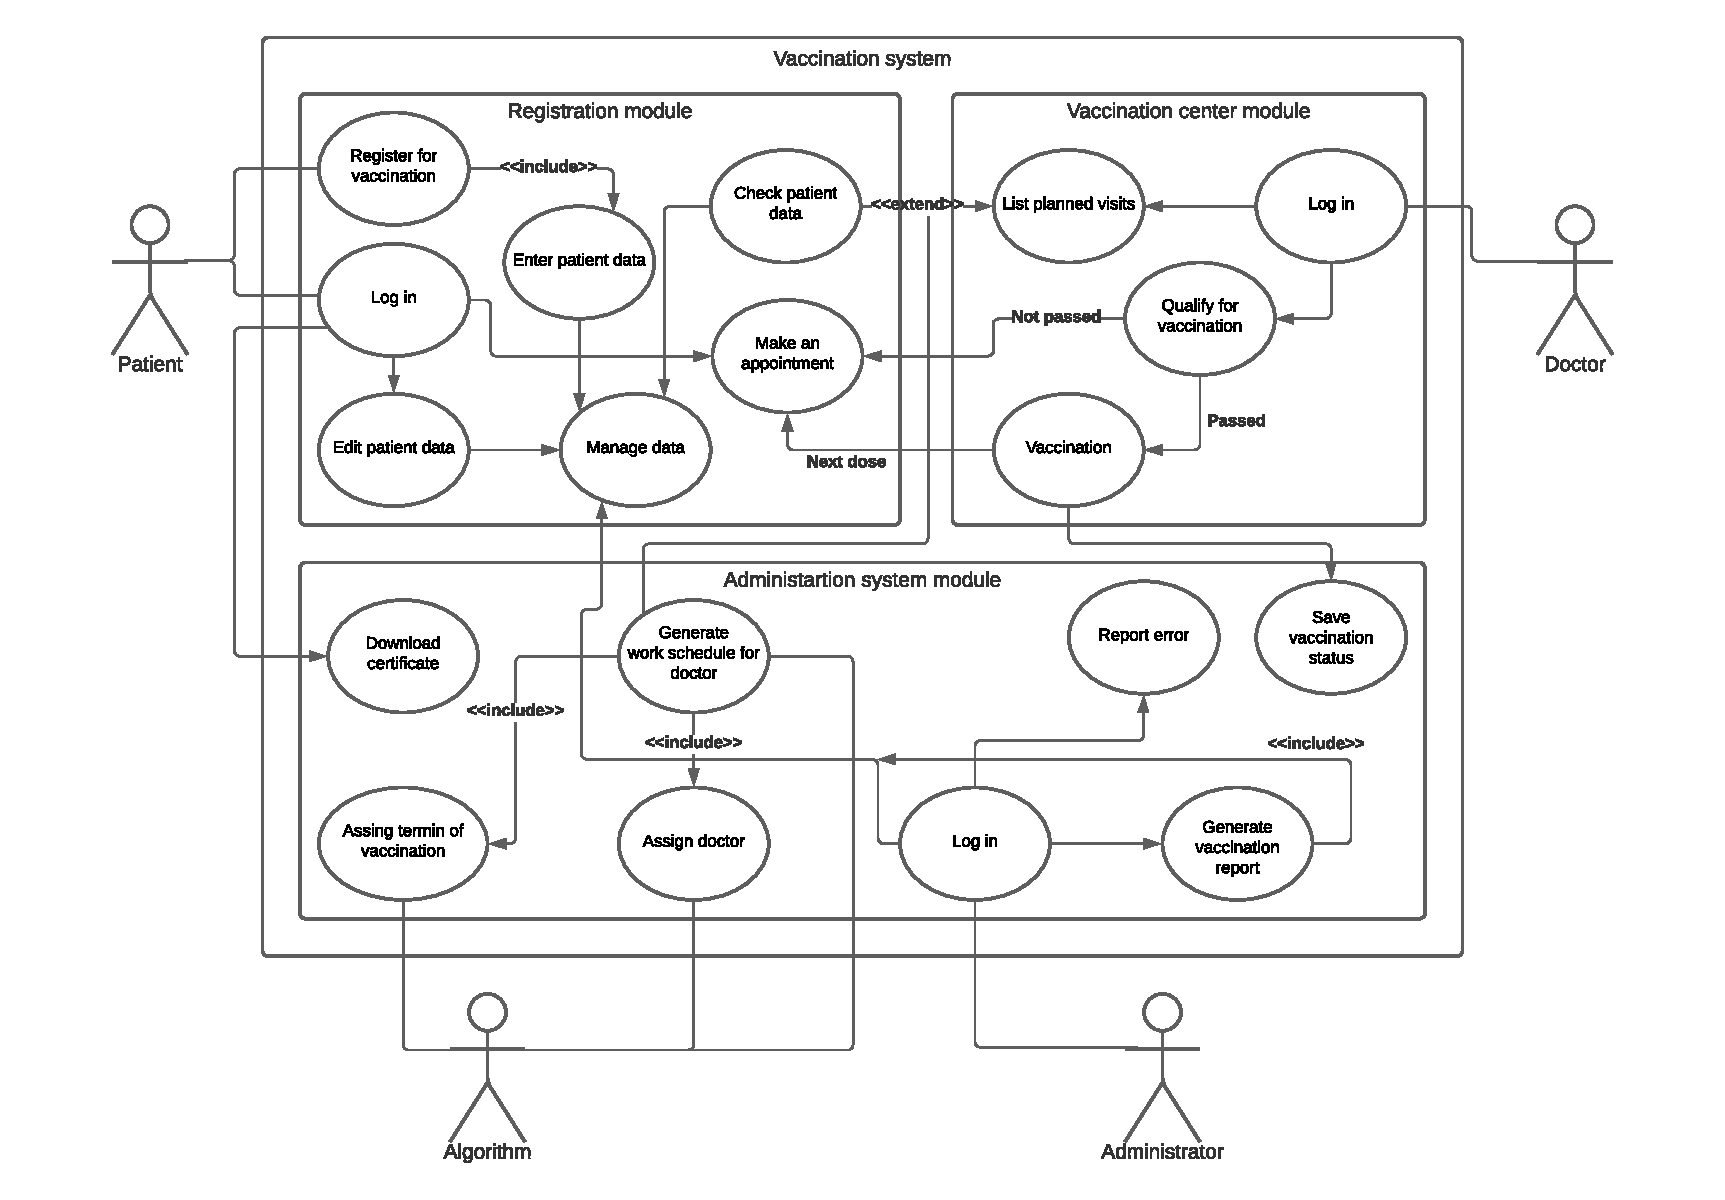
\includegraphics[width=\textwidth]{IO1 - diagram - ENG.pdf} 
    \caption{Diagram przypadków użycia \label{fig:diagram-uml}}
\end{figure}

Diagram przypadków użycia przedstawia główne funkcjonalności projektowanego systemu, jednocześnie odzwierciedlając przynależność danej funkcjonalności do konkretnego modułu. Aplikacja składa się z 3 głównych modułów opisanych w rozdziale 1.2. 

Aktorami w diagramie są
\begin{itemize}
    \item \texttt{Pacjent}, który ma bezpośredni dostęp do Modułu rejestracji.
    \item \texttt{Lekarz} połączony z modułem punktu szczepień.
    \item \texttt{Administrator} - osoba sprawująca opiekę nad całym systemem.
    \item \texttt{Algorytm} odpowiedzialny za optymalne przypisywanie pacjentów do szczepień oraz lekarzy.
\end{itemize}

Każdy aktor będący realnym klientem systemu (tzn. Pacjent, Lekarz i Administrator) łączy się z nim poprzez logowanie lub dodatkowo dla pacjenta poprzez krok Rejestracji na szczepienie.\\

Poniżej zostaną opisane kluczowe ścieżki użycia funkcjonalności dla konkretnych agentów:
\begin{itemize}
    \item \texttt{Pacjent}
    \begin{itemize}
        \item \texttt{Rejestracja na szczepienie}: użytkownik chcący zapisać się na szczepienie musi najpierw się zarejestrować i uzupełnić swoje dane.
        \item \texttt{Ustalenie terminu wizyty}: do ustalenia terminu wizyty potrzebna jest autoryzacja pacjenta.
        \item \texttt{Pobranie certyfikatu}: każdy zautoryzowany i zaszczepiony pacjent ma możliwość pobrania certyfikatu szczepienia.
    \end{itemize}
    \item \texttt{Lekarz} 
    \begin{itemize}
        \item \texttt{Wyświetlanie listy zaplanowanych wizyt}: zalogowany lekarz może pobrać listę wizyt przypisanych do niego w konkretnym dniu.
        \item \texttt{Kwalifikacja na szczepienie}: każdy pacjent przed przyjęciem szczepionki musi przejść przez kwalifikację. Jeśli lekarz stwierdzi, że pacjent jest niezdolny do przyjęcia szczepionki, to może go w następnym kroku zapisać na kolejną wizytę. W przypadku pozytywnej kwalifikacji, lekarz aplikuje szczepionkę i zapisuje status szczepienia w systemie. W przypadku, gdy szczepionka wymaga przyjęcia kilku dawek, lekarz jest też uprawiony do określenia terminu przyjęcia przez pacjenta kolejnej dawki.
    \end{itemize}
    \item \texttt{Administrator} 
    \begin{itemize}
        \item \texttt{Generacja raportów o szczepieniach}: zalogowany administrator może wygenerować raporty szczepień w celach analitycznych.
        \item \texttt{Zarządzanie danymi}: administrator ma możliwość modyfikacji danych zarówno pacjentów jak i lekarzy. Może także tworzyć konta dla nowych lekarzy.
        \item \texttt{Zgłaszanie błędu}: w przypadku wystąpienia błędu w systemie, administrator ma możliwość zgłoszenia go bezpośrednio do deweloperów.
     \end{itemize}
    \item \texttt{Algorytm}
    \begin{itemize}
        \item \texttt{Brak logowania}: w porównaniu z innymi aktorami algorytm nie ma kroku logowania, ponieważ algorytm jest programem, który stanowi integralną część systemu, więc nie musi się autoryzować.
        \item \texttt{Generacja grafików lekarzy}: algorytm zajmuje się optymalizacją grafików lekarzy. Ten przypadek użycia jest też rozdzielony na dwa mniejsze, które są w nim zawarte: Przydzielenie pacjentowi godziny szczepienia oraz Przydzielenie pacjentowi lekarza.
     \end{itemize}
\end{itemize}

\subsection{Diagram klas}
\begin{figure}[p]
    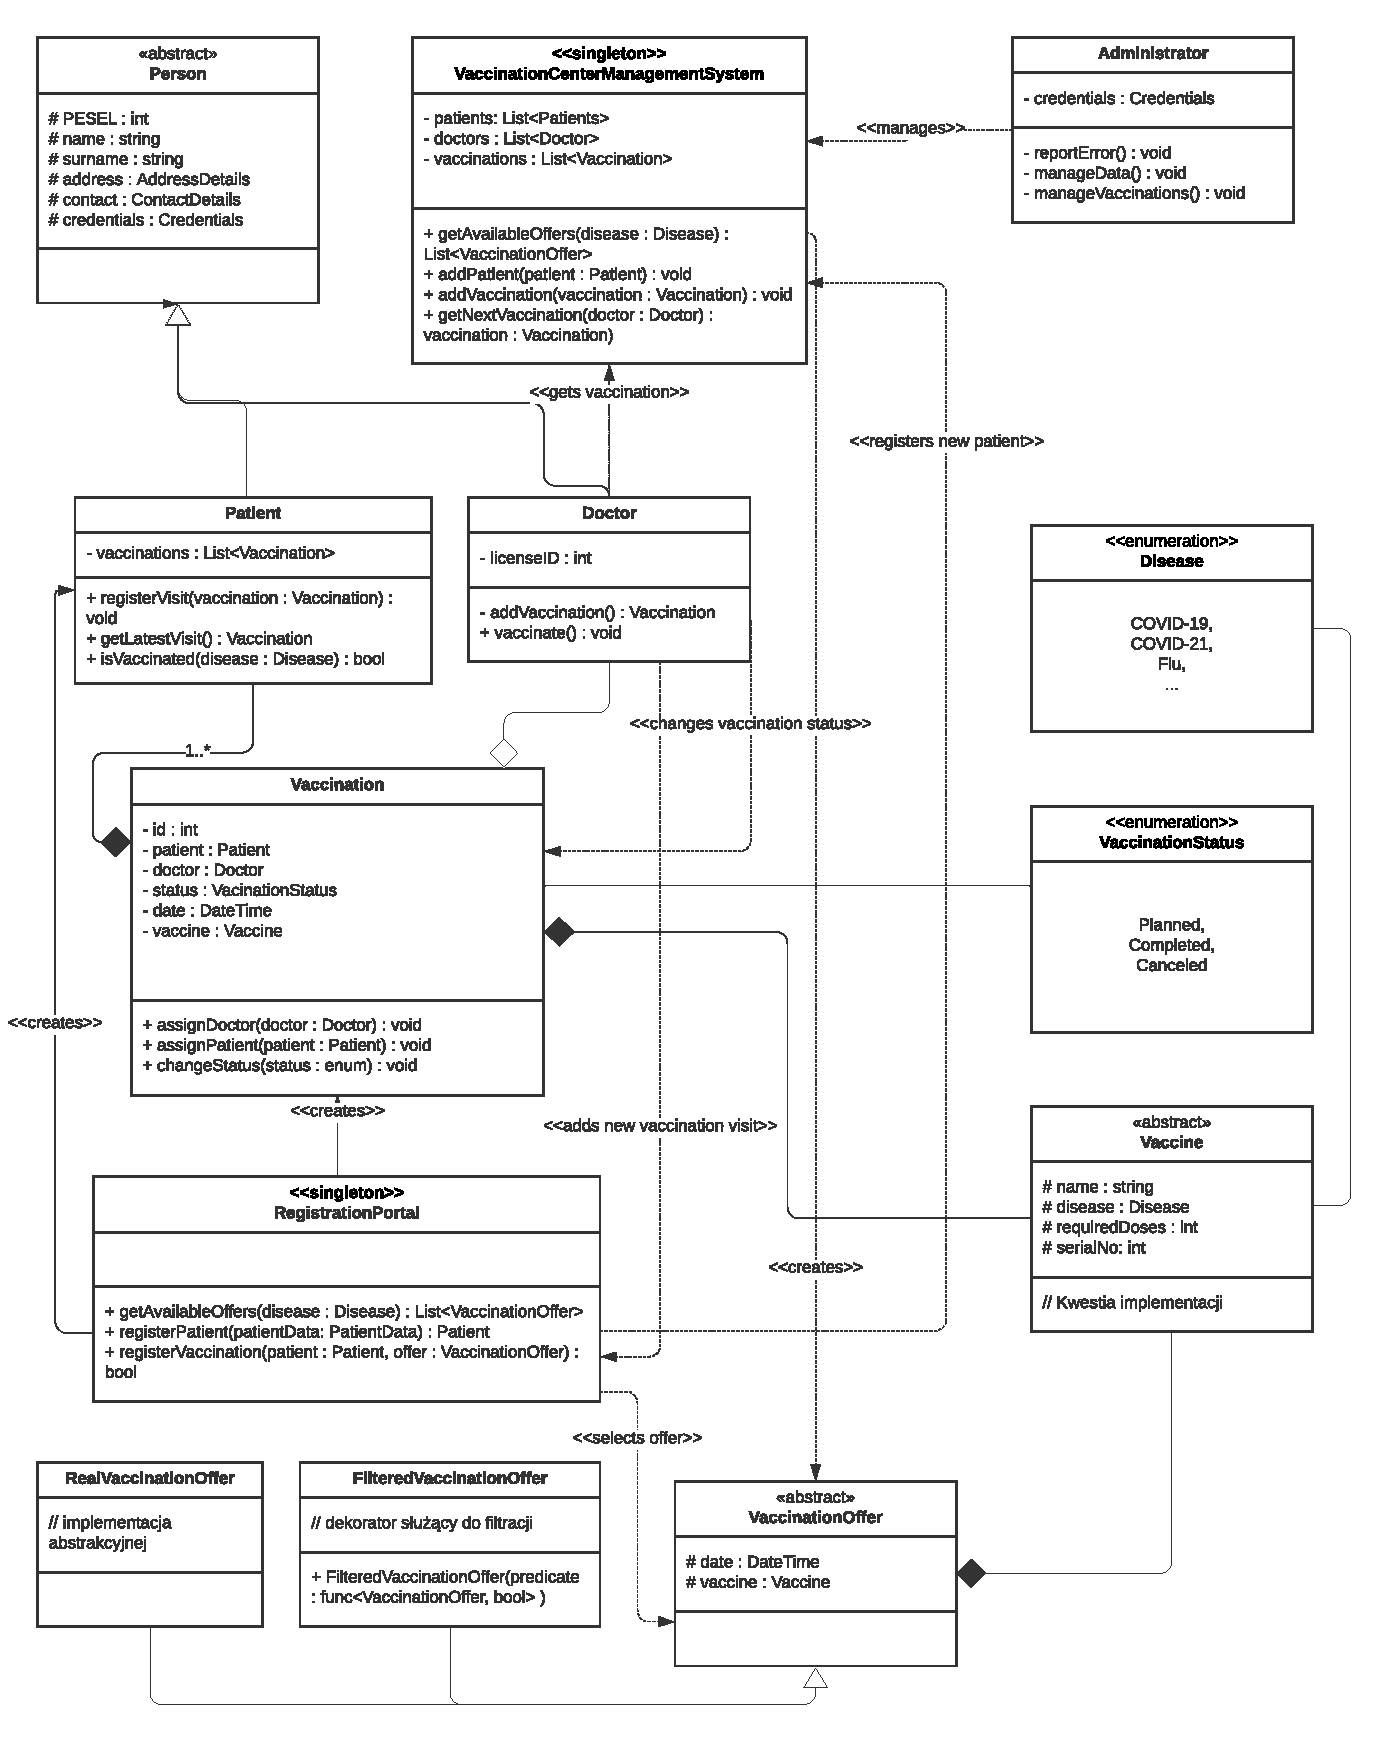
\includegraphics[width=\textwidth]{IO1 - diagram klas rev 2.0 (1).pdf} 
    \caption{Diagram klas \label{fig:diagram-uml}}
\end{figure}

Na diagramie klas przedstawione są kluczowe elementy systemu szczepień oraz najważniejsze powiązania między nimi: 
\begin{itemize}
    \item \texttt{RegistrationPortal}, za pomocą którego pacjenci rejestrują się i spośród przedstawionych im \texttt{VaccinationOffer} wybierają dogodną wizytę.
    \item \texttt{VaccinationCenterManagementSystem} pełniący rolę centralnej bazy danych.
    \item \texttt{Vaccination}, czyli poszczególne wizyty pacjentów - zarówno te zaplanowane, zakończone jak i odwołane - który zawiera wszystkie kluczowe informacje dotyczące danej wizyty, tj. odpowiedniego pacjenta, lekarza, wybraną szczepionkę, datę etc.
    \item \texttt{Patient}, agregujący dane pacjenta.
    \item \texttt{Doctor}, który przeprowadza faktyczne szczepienie.
    \item \texttt{Administrator} sprawujący opiekę nad systemem.
\end{itemize}

Oprócz nich na diagramie znajdują się też klasy służące do przechowywania odpowiednich danych:

\begin{itemize}
    \item \texttt{Person}, w której znajdują się dane osobowe i z której dziedzyczy \texttt{Patient} oraz \texttt{Doctor}.
    \item \texttt{Vaccine} opisująca szczepionkę na daną chorobę.
    \item \texttt{VaccinationOffer} będąca szkieletową wersją \texttt{Vaccination} służącą do przedstawienia pacjentowi możliwych terminów szczepień.
\end{itemize}

Algorytm odpowiedzialny za optymalne przydzielanie pacjentom godzin szczepień oraz konkretnych lekarzy jest w dużej mierze kwestią implementacji i powinien w szerokim zakresie współpracować z obiektem \texttt{VaccinationCenterManagementSystem}, zatem na diagramie nie zostały umieszczone szczegóły dotyczące jego projektu.

\newpage

\subsection{Kluczowe obiekty biznesowe}
System szczepień opiera się na trzech kluczowych obiektach biznesowych: pacjencie, szczepieniu i ofercie szczepień reprezentowanymi odpowiednio przez klasy Patient, Vaccination, Vaccination Offer.

Obiekt \texttt{Patient} zawiera dane pacjenta, który korzysta z systemu szczepień, jak również całą jego historię szczepień zapisaną w postaci listy obiektów \texttt{Vaccination}. Obiekt ten zawiera również dane logowania umożliwiające skorzystanie z modułu rejestacji.

Obiekt \texttt{Vaccination} jest podstawowym obiektem służącym do zapisu informacji o pojedynczej wizycie. W trakcie rejestracji i oczekiwania na wizytę służy jako informacja o nadchodzącym szczepieniu, zaś po wykonaniu zabiegu służy jako rekord potwierdzający fakt zaszczepienia.

Obiekt \texttt{VaccinationOffer} jest uproszczoną wersją obiektu Obiekt \texttt{Vaccination}, która jest wykorzystywana przez system do udostępnienia rejestrującemu się pacjentowi listy możliwych terminów szczepień. 

\newpage

\subsection{Diagram stanów}
Diagramy stanów przedstawiają cykl życia kluczowych obiektów biznesowych wykorzystywanych przez system szczepień oraz przejścia powodujące zmiany ich stanów.

\subsubsection{Pacjent}
\begin{figure}[h]
    \includegraphics[width=\textwidth]{IO1 - diagram stanów - Patient.pdf} 
    \caption{Diagram stanów obiektu Patient \label{fig:diagram-uml}}
\end{figure}
Obiekt \texttt{Patient} jest tworzony po otwarciu przez pacjenta formularza rejestracyjnego. Początkowym stanem tego obiektu jest stan \textit{Registering}. Po przesłaniu formularza wprowadzane dane są weryfikowane, sprawdzane jest m.in. czy wszystkie pola zostały wypełnione i czy wprowadzony numer PESEL jest poprawny. W przypadku gdy weryfikacja na dowolnym z etapów się nie powiedzie, obiekt powraca do stanu \textit{Registering}, w którym pacjent ma możliwość edycji i poprawy danych wprowadzonych w formularzu.
W razie rezygnacji z rejestracji (tj. zamknięcia przez pacjenta formularza) obiekt jest niszczony.

W przypadku gdy formularz zostanie przesłany i weryfikacja zakończy się pomyślnie, obiekt przechodzi w stan \textit{Idle}, w którym pacjent ma możliwość sprawdzenia swojej historii szczepień oraz rozpoczęcia procesu zapisu na szczepienie.

Rozpoczęcie procesu rejestracji na szczepienie powoduje przejście obiektu ze stanu \textit{Idle} na \textit{Choosing vaccination offer}. Pacjent ma możliwość wybrania jednej z przedstawionych przez system ofert szczepień. Jeżeli pacjent wybierze ofertę, następuje rejestracja na szczepienie, po czym obiekt wraca do stanu \textit{Idle}. W przypadku rezygnacji z rejestracji na szczepienie, obiekt powraca do stanu \textit{Idle} bez wykonywania żadnych akcji.

Jeżeli pacjent zażąda usunięcia swojego konta, obiekt przechodzi ze stanu \textit{Idle} na stan \textit{Archived} (stan finalny), zaś pacjent otrzymuje potwierdzenie wykonania akcji. W tym stanie konto pacjenta zostaje zarchiwizowane i nie jest już dłużej aktywne.

\subsubsection{Oferta szczepienia}

\begin{figure}[h]
    \centering
    \includegraphics[scale=0.7]{IO1 - diagram stanów - VaccinationOffer.pdf} 
    \caption{Diagram stanów obiektu VaccinationOffer \label{fig:diagram-uml}}
\end{figure}

Obiekt \texttt{Vaccinationoffer} jest tworzony po rozpoczęciu przez pacjenta procesu rejestracji na szczepienie i zawiera jedną z ofert szczepienia wygenerowaną przez system. Początkowym stanem tego obiektu jest stan \textit{Available offer}. Jeżeli oferta zostanie wybrana przez pacjenta, obiekt przechodzi do stanu \textit{Chosen offer}, gdzie następuje rejestracja na szczepienie. Jeżeli oferta nie zostanie wybrana, obiekt przechodzi do stanu \textit{Canceled offer} bez wykonywania żadnych akcji. Po wykonaniu ewentualnych czynności w stanach \textit{Chosen offer} i \textit{Canceled offer} obiekt jest niszczony.

\newpage

\subsubsection{Szczepienie}
\begin{figure}[h]
    \includegraphics[width=\textwidth]{IO1 - diagram stanów - Vaccination.pdf} 
    \caption{Diagram stanów obiektu Vaccination
    \label{fig:diagram-uml}}
\end{figure}
Obiekt \texttt{Vaccination} jest tworzony po rejestracji przez pacjenta na wybrany termin szczepienia. Początkowym stanem tego obiektu jest stan \textit{Awaiting doctor}, w którym ustalony jest już termin i rodzaj szczepionki, ale do wizyty nie jest jeszcze przypisany przez system żaden lekarz. W momencie gdy nadejdzie czas szczepienia, a obiekt będzie znajdował się w stanie \textit{Awaiting doctor}, wizyta zostanie anulowana, zaś obiekt przejdzie w stan \textit{Canceled}.


W momencie gdy system przypisze lekarza do wizyty, obiekt przechodzi do stanu \textit{Planned}, w którym wysyłane jest do pacjenta potwierdzenie wizyty. Gdy nadejdzie termin wizyty weryfikowana jest obecność pacjenta w punkcie szczepień. Jeżeli pacjent jest obecny, następuje jego kwalifikacja do szczepienia. Jeżeli  przejdzie on kwalifikację, to zostaje zaszczepiony, zaś obiekt przechodzi w stan \textit{Completed}. Jeżeli pacjent nie pojawi się lub nie przejdzie kwalifikacji, to obiekt przechodzi w stan \textit{Canceled}, a zabieg nie jest wykonywany.

Gdy obiekt znajduje się w stanach \textit{Awaiting doctor} lub \textit{Planned}, pacjent ma możliwość anulowania wizyty. Obiekt przechodzi wtedy w stan \textit{Canceled}. Po wykonaniu czynności w stanach \textit{Completed} i \textit{Canceled} obiekt przechodzi w stan finalny.

\newpage

\subsection{Diagram aktywności}
Diagramy aktywności przedstawiają ścieżki wykonania kluczowej funkcjonalności systemu jaką jest proces szczepienia pacjenta - od rejestracji wizyty, przez wizytę w punkcie szczepień, po czynności administracyjne po wykonaniu zabiegu.

\begin{figure}[h]
    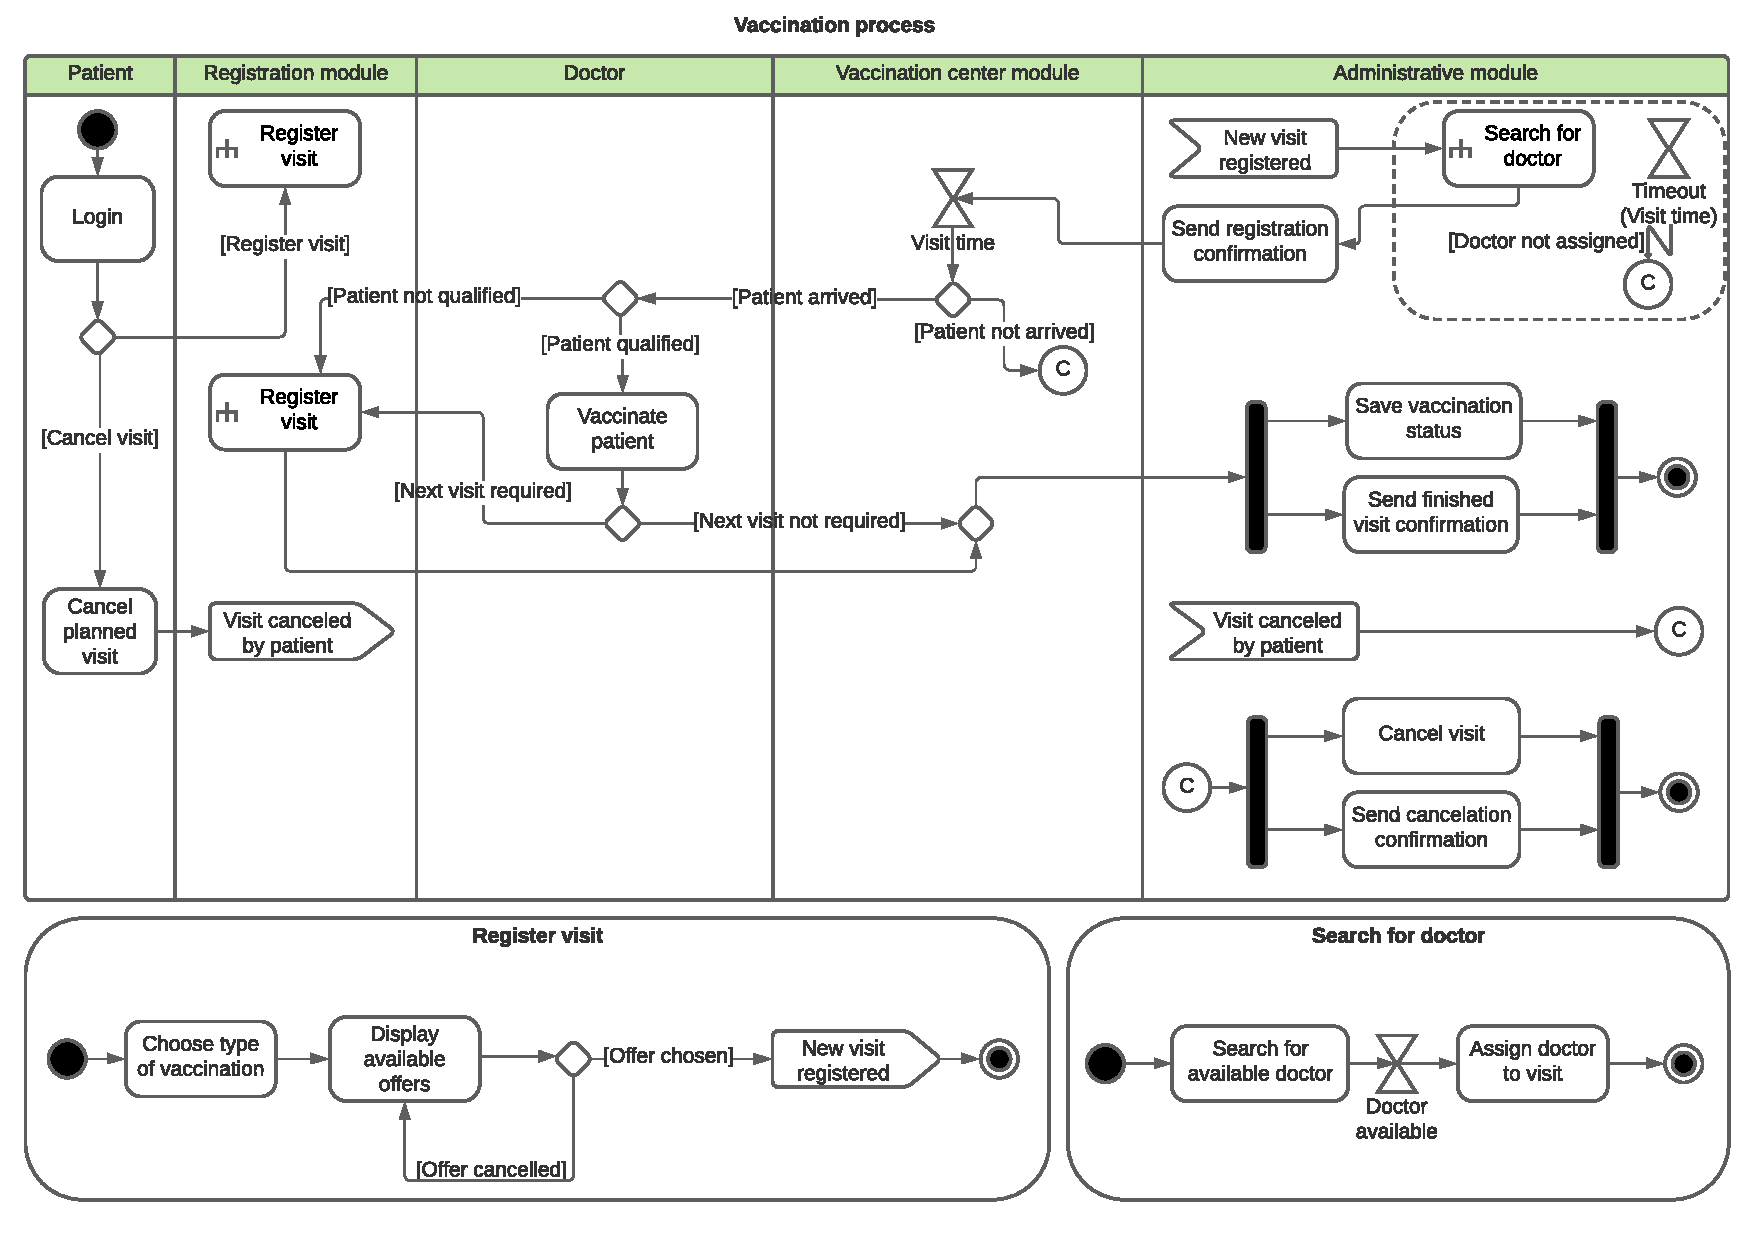
\includegraphics[width=\textwidth]{IO1 - diagram aktywnosci.pdf} 
    \caption{Diagram aktywności procesu szczepienia
    \label{fig:diagram-uml}}
\end{figure}

\subsubsection{Proces szczepienia}
Pierwszy krok w procesie szczepienia jest inicjowany przez pacjenta przez zalogowanie się w module rejestracji. Pacjent może zarejestrować się na nową wizytę (zgodnie z opisaną w następnym podpunkcie procedurą) lub odwołać zaplanowaną wcześniej wizytę.

W przypadku rejestracji na nową wizytę wykonywane akcje są zgodne z procedurą \textit{Register visit}, wysyłającą sygnał \textit{New visit registered}, na który oczekuje moduł administracyjny. Po otrzymaniu tego sygnału moduł przystępuje do wyszukiwania i przydzielania dostępnego lekarza zgodnie z procedurą \textit{Search for doctor}. W przypadku gdy w wyznaczonym czasie nie zostanie znaleziony dostępny lekarz wizyta zostaje anulowana. Po znalezieniu lekarza system wysyła potwierdzenie rejestracji, zaś moduł punktu szczepień rozpoczyna oczekiwanie na czas wizyty.

Po nadejściu czasu wizyty moduł punktu szczepień dokonuje sprawdzenia, czy pacjent stawił się na wizytę. W przypadku, gdy pacjent nie pojawił się na czas wizyta zostaje anulowana. Jeżeli pacjent stawił się w punkcie szczepień, lekarz przystępuje do kwalifikacji na szczepienie. W przypadku, gdy pacjent nie zakwalifikuje się do zabiegu, lekarz wyznacza mu nowy termin wizyty zgodnie z procedurą rejestracji na wizytę. Jeżeli pacjent zostanie zakwalifikowany pozytywnie, lekarz przystępuje do wykonania zabiegu, po czym w zależności od potrzeb może również wyznaczyć termin następnej wizyty (przykładowo gdy wymagane jest podanie kolejnej dawki szczepionki). Następnie w module administracyjnym zapisywany jest aktualny status szczepienia i wysyłane jest potwierdzenie zakończonej wizyty.

W przypadku anulowania wizyty, moduł rejestracji wysyła sygnał \textit{Visit canceled by patient}, który jest odbierany przez moduł administracyjny, który dokonuje anulowania wizyty i wysyła pacjentowi potwierdzenie anulowania.

\subsubsection{Procedura rejestracji na wizytę}
Podczas procedury rejestracji na wizytę pacjent wybiera z pomocą modułu rejestracji rodzaj choroby, na którą chciałby się zaszczepić, po czym otrzymuje listę dostępnych ofert, spośród których może wybrać tą, która najbardziej mu odpowiada. Jeżeli pacjent wybierze ofertę, moduł rejestracji wysyła sygnał \textit{New visit registered}, po czym procedura się kończy. Jeżeli pacjent zrezygnuje z wyboru oferty, będzie on mógł wrócić do listy dostępnych ofert i wybrać inną.

\subsubsection{Procedura wyszukiwania i przydzielania dostępnego lekarza}
Procedura wyszukiwania i przydzielania dostępnego lekarza wyszukuje z pomocą modułu administracyjnego lekarza, który mógłby wykonać szczepienie w wybranym przez pacjenta terminie. Moduł administracyjny oczekuje na dostępność lekarza, po czym przydziela go do rozważanej wizyty, po czym procedura kończy działanie. Moduł administracyjny może przerwać tą procedurę po upływie ustalonego czasu.

\newpage

\subsection{Diagram sekwencji}
Wszystkie diagramy sekwencji oparte są o podział Użytkownik - Aplikacja (frontend) - Serwer (backend / baza danych).

\subsubsection{Zarządzenie kontem pacjenta}

\begin{figure}[!h]
    \centering
    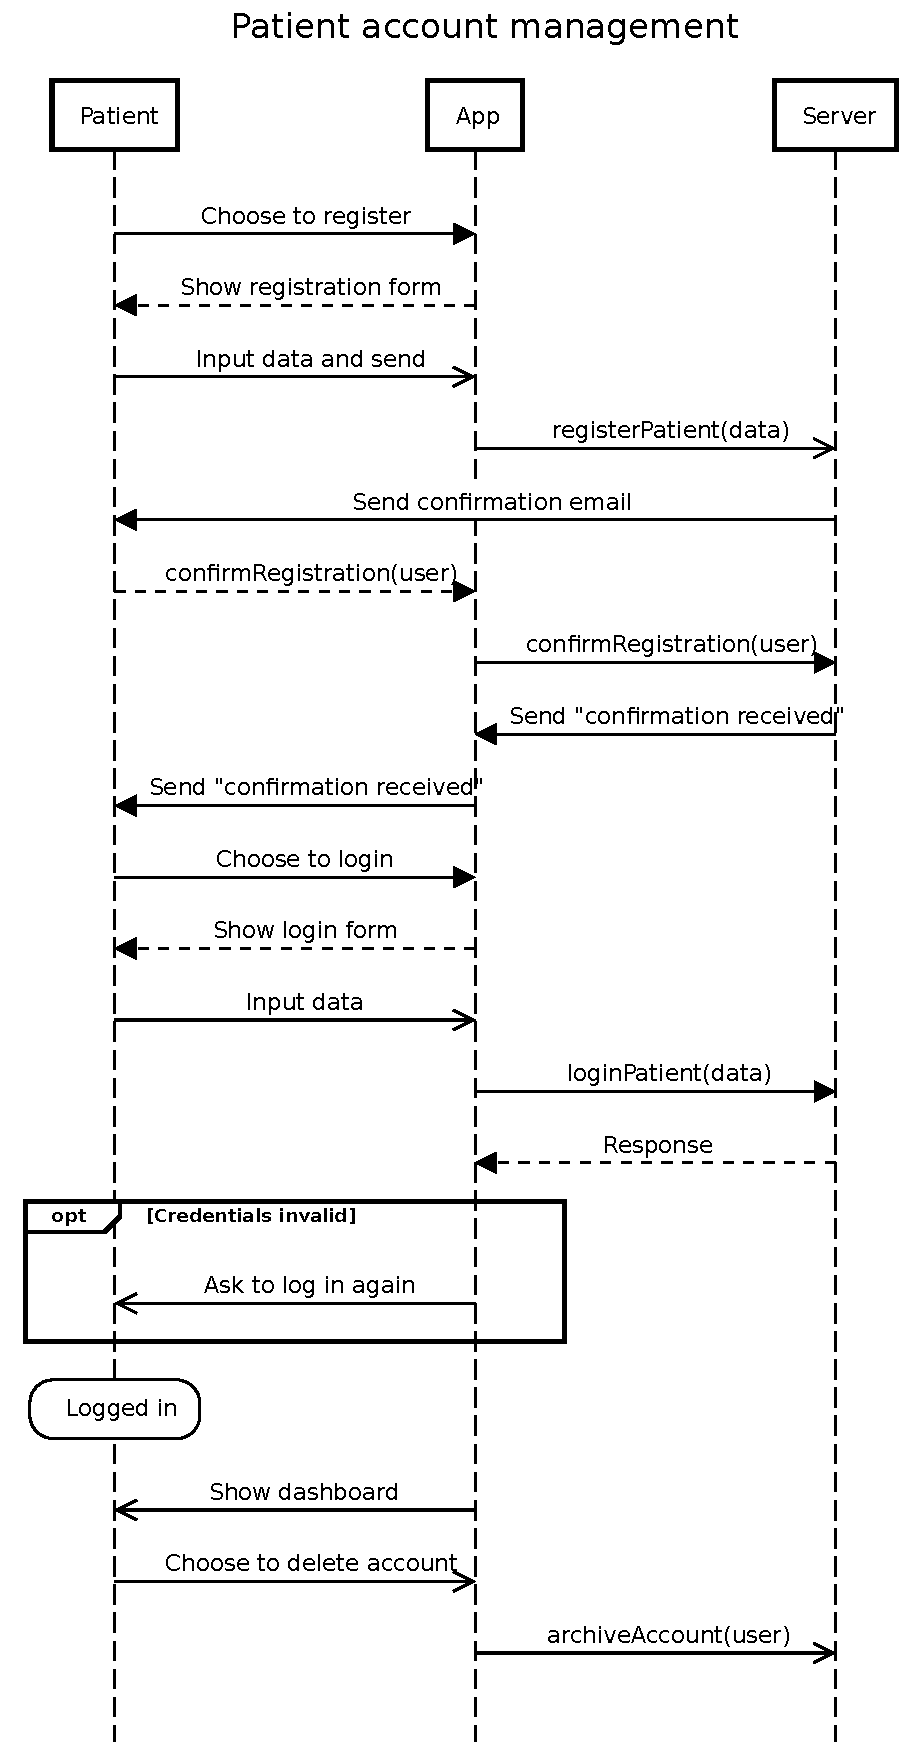
\includegraphics[width=\textwidth,height=0.6\textheight,keepaspectratio]{Patient_account_management.pdf} 
    \caption{Diagram sekwencji zarządzania kontem pacjenta
    \label{fig:diagram-uml}}
\end{figure}
Diagram zarządzania kontem pacjenta pokazuje, jak wygląda komunikacja między aplikacją a serwerem w odpowiedzi na żądania użytkownika, który przechodzi przez kolejne etapy tworzenia swojego konta. Serwer odpowiada na zapytania dotyczące zarejestrowania nowej osoby w bazie danych, wysyła odpowiedni mail aktywacyjny, umożliwia faktyczne zalogowanie w systemie i zarchiwizowanie konta. Reszta funkcjonalności, np. ewentualnie sprawdzenie poprawności danych, pokazywanie odpowiednich formularzy, etc. leży po stronie aplikacji, z którą użytkownik wchodzi w interakcję.

\newpage
\subsubsection{Szczepienie}

\begin{figure}[!h]
    \centering
    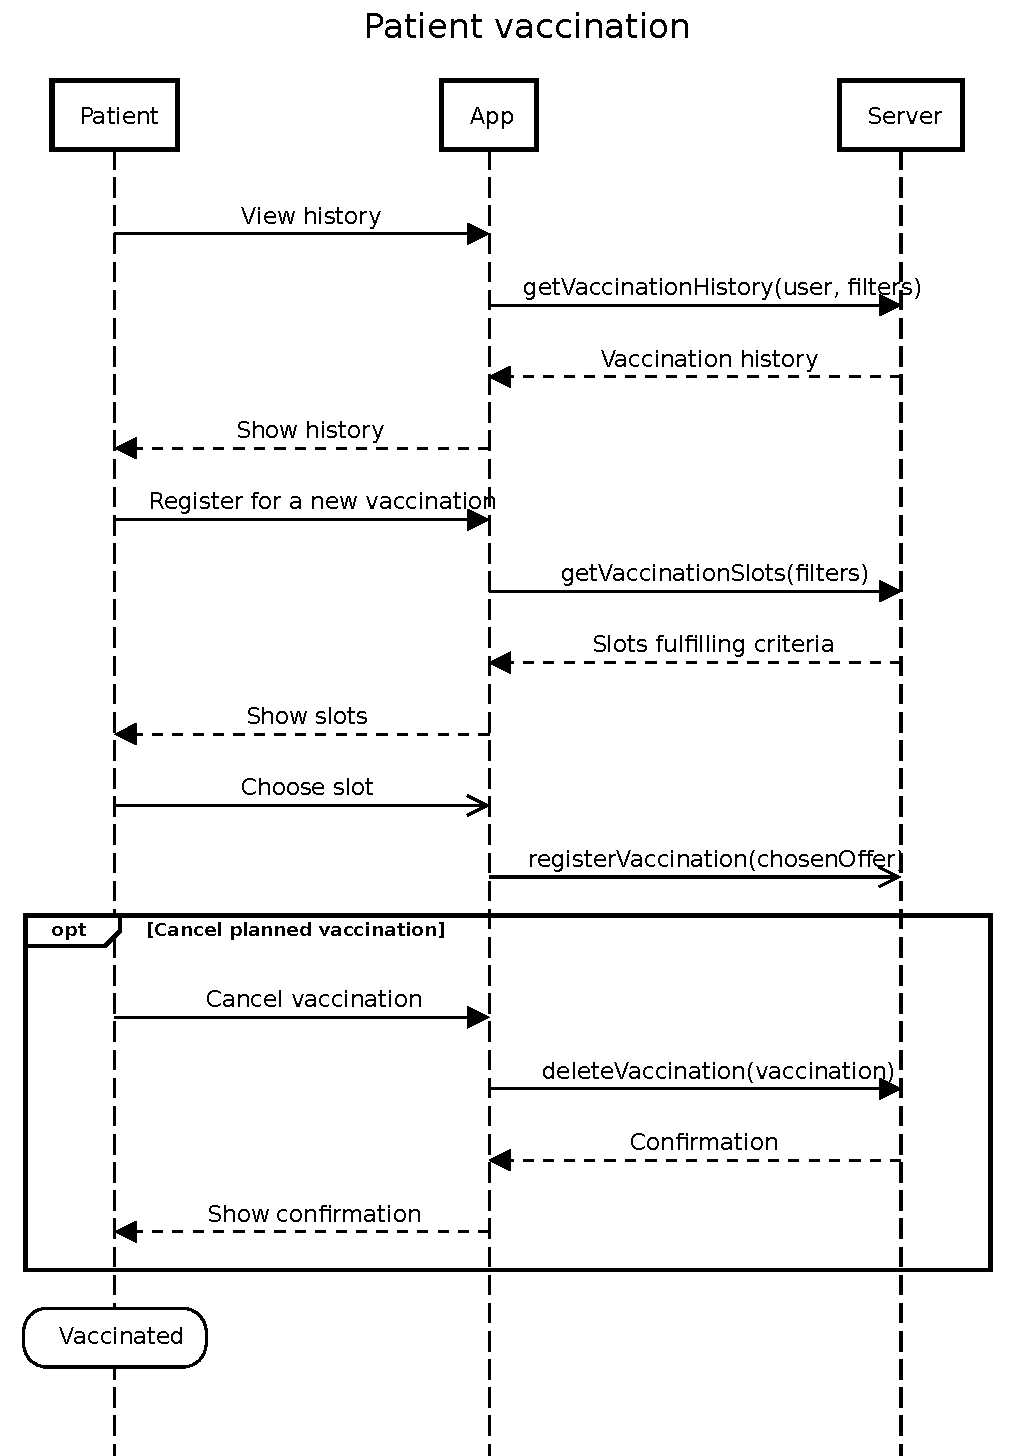
\includegraphics[width=\textwidth,height=0.7\textheight,keepaspectratio]{Patient_vaccination.pdf} 
    \caption{Diagram sekwencji procesu szczepienia
    \label{fig:diagram-uml}}
\end{figure}
Na tym diagramie widać, jak przebiega proces rejestracji na nowe szczepienie. Po uprzednim zalogowaniu w systemie użytkownik może sprawdzić historię swoich poprzednich wizyt, również z możliwością filtracji wg. odpowiednich kryteriów, a następnie przejść do formularza rejestracyjnego. System odsyła wolne terminy dla szczepień, które interesują użytkownika, spośród których ten może dokonać najlepszego dlań wyboru. Możliwe jest również anulowanie zaplanowanej wizyty - w takim przypadku na odpowiednie żądanie system odsyła potwierdzenie wykonania zlecenia.

\newpage

\subsubsection{Praca lekarza}

\begin{figure}[!htbp]
    \centering
    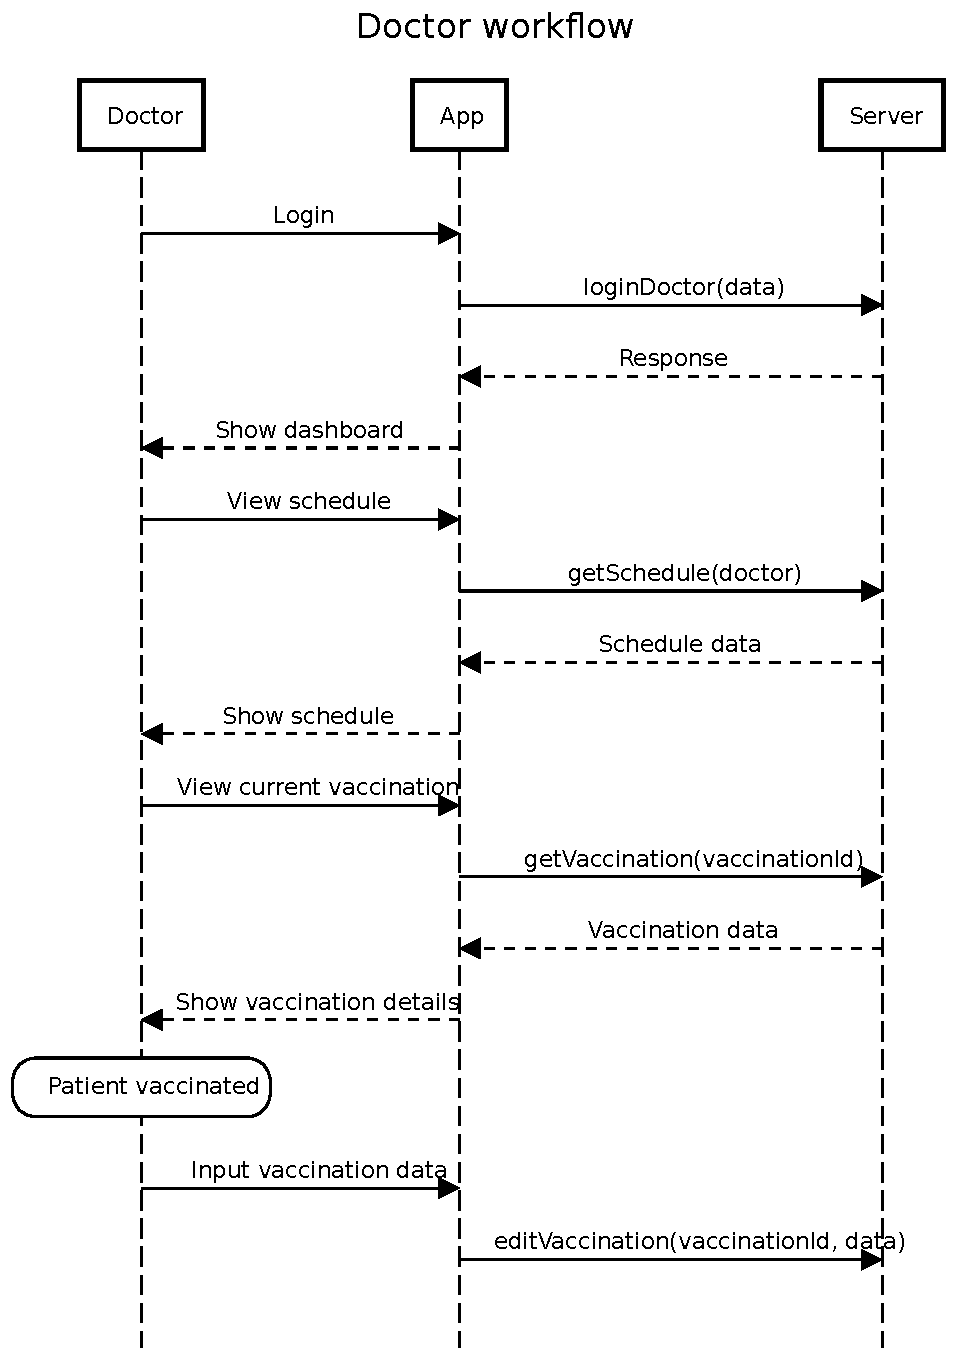
\includegraphics[width=\textwidth,height=0.7\textheight,keepaspectratio]{Doctor_workflow.pdf} 
    \caption{Diagram sekwencji pracy lekarza
    \label{fig:diagram-uml}}
\end{figure}
Diagram opisuje, jak wygląda wycinek pracy lekarza od momentu zalogowania w systemie do momentu zapisania nowego szczepienia - po sprawdzeniu swojego grafiku na dany dzień, lekarzowi po kolei wyświetlają się dane poszczególnych zaplanowanych wizyt. Po wykonaniu szczepienia lekarz wpisuje odpowiednie dane do udostępnionego mu formularza, które są następnie zapisywane do systemu.

\newpage

\subsubsection{Praca administratora}

\begin{figure}[!htbp]
    \centering
    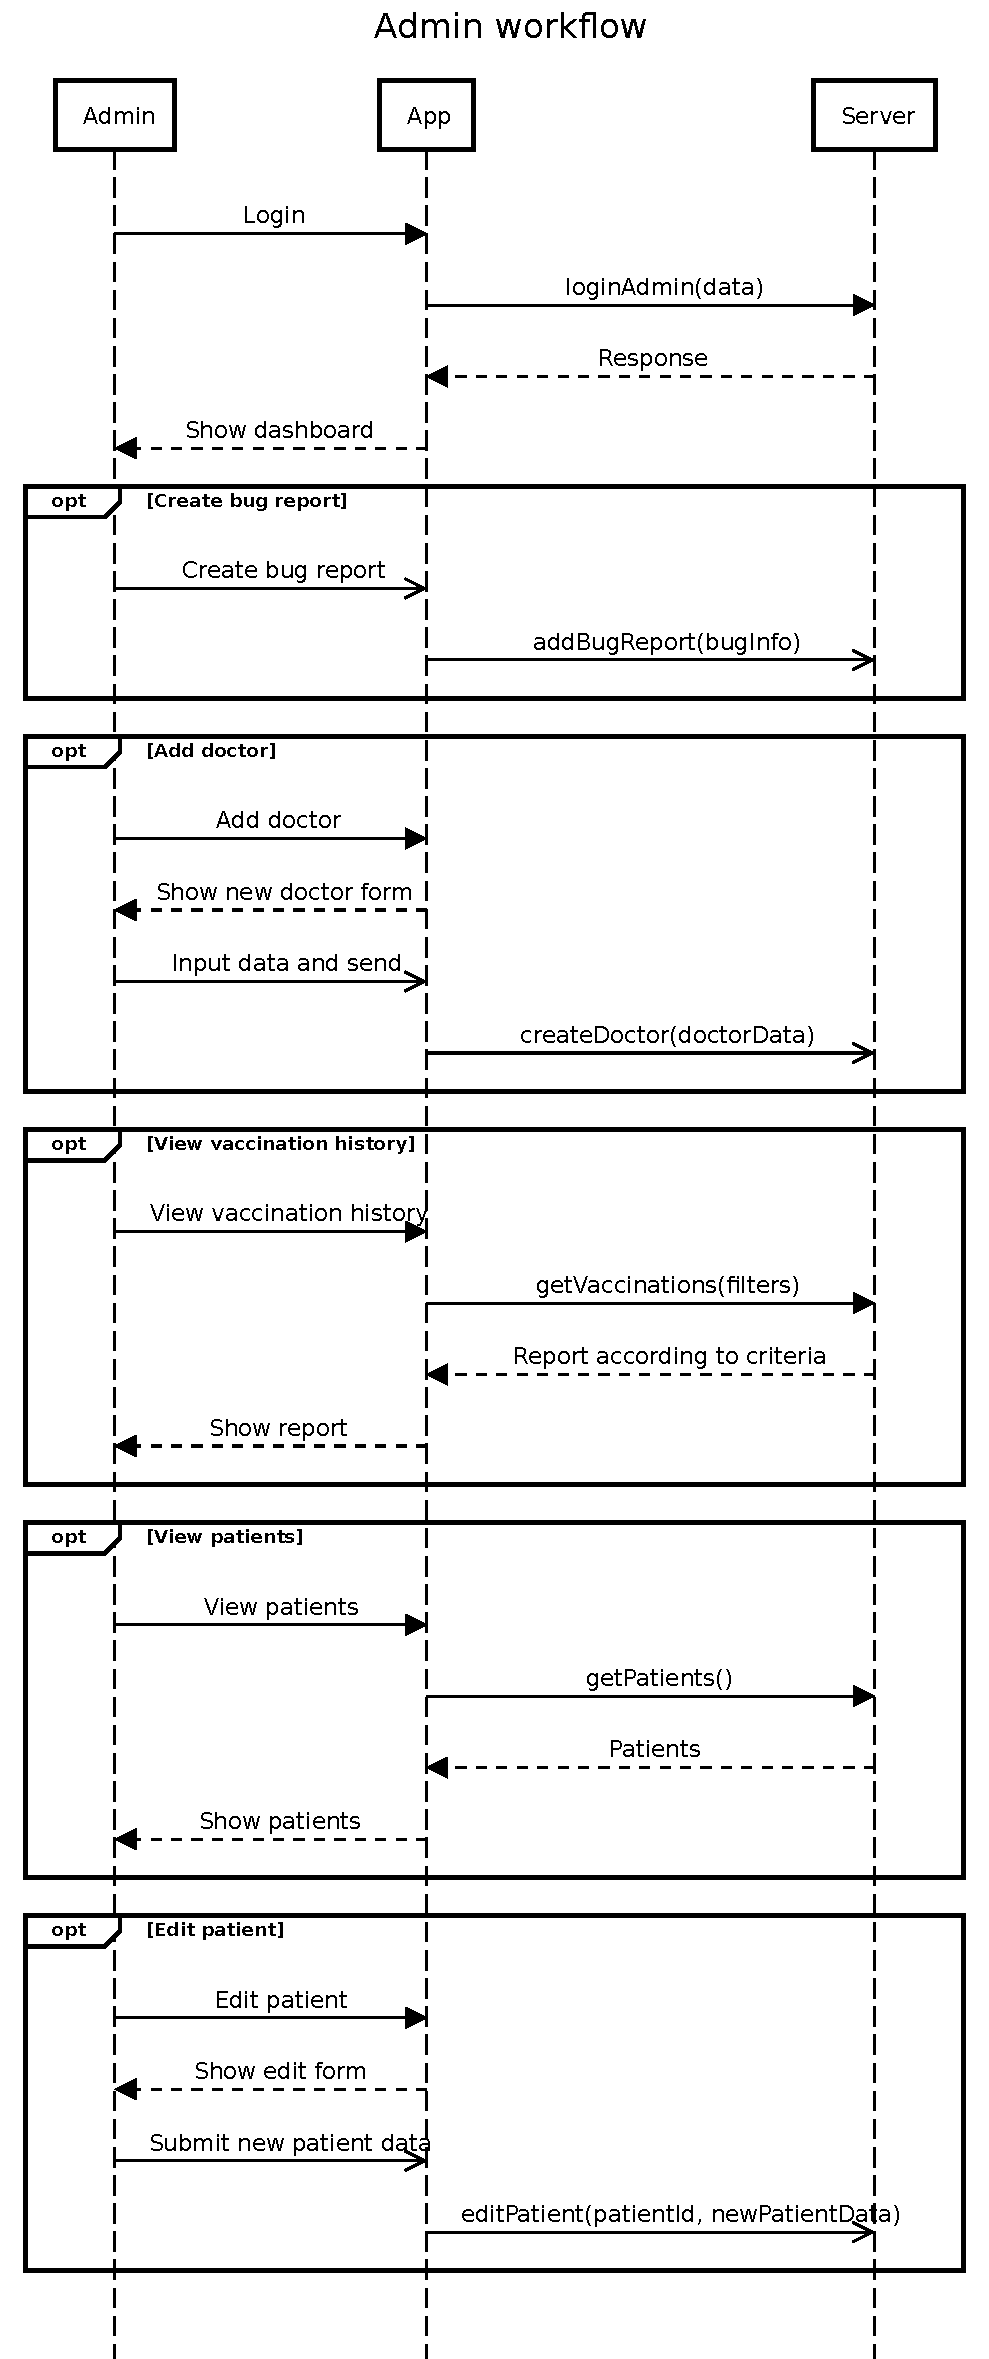
\includegraphics[width=\textwidth,height=0.8\textheight,keepaspectratio]{Admin_workflow.pdf} 
    \caption{Diagram sekwencji pracy administratora
    \label{fig:diagram-uml}}
\end{figure}
Diagram z administratorem pokazuje, jakich akcji może on dokonać w systemie oraz jak przebiegają związane z nimi procesy. Administrator ma dostęp do CRUD'a zarówno dla pacjentów, jak i doktorów, może zapisywać w systemie sprawozdania z błędów do obsługi przez dział IT oraz generować rozmaite raporty na podstawie danych ze szczepień.

\newpage

\subsubsection{Pobieranie certyfikatu szczepienia}
\begin{figure}[h]
    \centering
    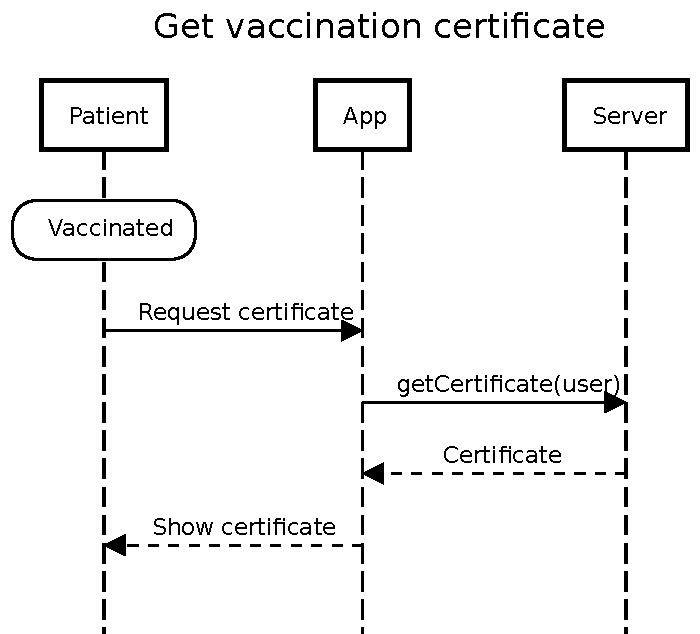
\includegraphics[width=0.5\textwidth,keepaspectratio]{Get_vaccination_certificate.pdf} 
    \caption{Diagram sekwencji pobierania certyfikatu szczepienia
    \label{fig:diagram-uml}}
\end{figure}

Diagram obrazuje prostą interakcję, która zachodzi w przypadku, kiedy użytkownik systemu pragnie pobrać certyfikat szczepień, które odbył.

\subsection{Dokumentacja API}
Dokumentacja API wykorzystywanego w systemie została opisana w załącznikach do niniejszej specyfikacji:
\begin{itemize}
    \item admin.html,
    \item doctor.html,
    \item patient.html.
\end{itemize}
Do każdego z powyższych plików zostały również dołączone źródła w formacie OpenAPI.

\section{Algorytmy biznesowe}
W rozważanym systemie szczepień szczególne znaczenie ma algorytm odpowiadający za przydzielenie lekarza do zaplanowanej wizyty.

\subsection{Założenia algorytmu}
Z perspektywy trwającego procesu szczepień najwyższym priorytetem jest zapewnienie pacjentom możliwości zaszczepienia się w dogodnym, możliwie najszybszym terminie, dlatego wykorzystany algorytm na pierwszym miejscu powinien skupić się na umożliwieniu rejestrację na wizytę jeśli tylko możliwe jest znalezienie lekarza na ten termin. Dopiero na kolejnym miejscu znajdować powinna się kwestia optymalnego wykorzystania czasu lekarzy i optymalnego dobrania wielkości personelu pracującego w danym dniu.

Z punktu widzenia systemu szczepień dopuszczalne jest zastosowanie algorytmu o naturze hybrydowej - tj. stosującego nieoptymalną strategię w celu przypisania lekarzy do poszczególnych terminów na bieżąco, w miarę kolejnych rejestracji (przykładowo przy pomocy podejścia zachłannego), a następnie wykonaniu co określony czas reorganizacji grafiku przy zastosowaniu optymalniejszej strategii. Przy zastosowaniu takiego podejścia należy jednak zagwarantować brak przerw w działaniu systemu oraz przezroczystość procesu z perspektywy pacjenta, który nie zna lekarza przypisanego do swojej wizyty. W szczególności nie może dojść do sytuacji, w której przy optymalizacji grafiku pacjent straci lekarza przypisanego do swojego terminu, a w konsekwencji jego wizyta zostanie anulowana.

\subsection{Referencyjna implementacja}
\textit{Krok 1.} Algorytm otrzymuje prośbę o przydzielenie lekarza do wizyty, która odbędzie się w podanym terminie.\\
\textit{Krok 2.} Algorytm pobiera listę lekarzy pracujących w punkcie szczepień, którzy są dostępni w podanym terminie.\\
\textit{Krok 3.} Jeżeli w wyniku działania kroku 2. znaleziono więcej niż jednego lekarza, algorytm wybiera lekarza, dla którego pozostałe wizyty są najbliżej podanego terminu - co jest rozumiane jako różnica czasu zakończenia ostatniej wizyty przed podanym terminem i czasu rozpoczęcia aktualnie rozważanej wizyty lub różnica czasu zakończenia rozważanej wizyty i czasu rozpoczęcia pierwszej wizyty po podanym terminie.\\
\textit{Krok 4.} Jeżeli w wyniku działania kroku 3. znaleziono więcej niż jednego lekarza, algorytm wybiera lekarza, który w danym dniu ma przypisaną większą liczbę wizyt.\\
\textit{Krok 5.} Jeżeli w wyniku działania kroku 4. znaleziono więcej niż jednego lekarza, algorytm wybiera pierwszego lekarza z przedstawionej listy kandydatów.\\
\textit{Krok 6.} Jeżeli w wyniku działania kroku 2. nie odnaleziono żadnego lekarza, algorytm rozpoczyna oczekiwanie na pojawienie się dostępnych lekarzy, po czym wraca do rozważań z kroku 2. Oczekiwanie może zostać przerwane przez czynnik zewnętrzny (moduł administracyjny) po upływie zdefiniowanego maksymalnego czasu oczekiwania.\\
\textit{Krok 7.} Jeżeli w wyniku działania powyższych procedur został wyznaczony lekarz, jest on zwracany przez algorytm.\\

\newpage

\section{Wymagania techniczne}
\subsection{Wymagania systemu}
Ze względu na zakładaną powszechną dostępność systemu szczepień komponenty wykorzystywane przez użytkowników końcowych (\textit{frontend}) powinny zostać zaimplementowane w formie aplikacji internetowych, które będą poprawnie działały na aktualnych wersjach najpopularniejszych przeglądarek internetowych (Google Chrome, Edge, Firefox, Opera) oraz przeglądarek internetowych na urządzeniach mobilnych (Google Chrome, Safari).

Ze względów praktycznych (dostępność systemów i komputerów do testowania i uruchomienia aplikacji) silnik systemu szczepień (\textit{backend}) powinien zostać zaimplementowany w formie programu działającego na systemie Windows 10 (lub nowszym) oraz Windows Server 2019 (lub nowszym). Obsługa innych systemów operacyjnych (wynikająca przykładowo z zastosowania technologi multiplatformowej) jest opcjonalna.

\subsection{Preferowane technologie}
Przy implementacji systemu szczepień proponowane jest wykorzystanie jednego z popularnych frameworków frontendowych takich jak React, Vue lub Angular, zaś w przypadku backendu jednego z frameworków takich jak ASP.NET (C\#), Spring (Java), Laravel (PHP) i podobne. 

Wśród dostępnych technologii preferowane (ale nie wymagane) jest wykorzystanie frameworka Vue dla frontendu, zaś ASP.NET do backendu. Za wyborem tych technologii stoi kilka istotnych czynników, takich jak:
\begin{itemize}
    \item dobra znajomość języków JavaScript i C\# wśród grupy programistów (studentów MiNI) zajmujących się implementacją systemu,
    \item popularność frameworków Vue oraz ASP.NET oraz ich dobra dokumentacja,
    \item duża liczba zewnętrznych bibliotek do wyżej wymienionych frameworków,
    \item dobra integracja języka C\# z innymi preferowanymi narzędziami firmy Microsoft (chmura Azure, baza danych MS-SQL),
    \item spójność środowiska .NET i dostępne narzędzia ułatwiające szybkie stworzenie rozważanego systemu, wsparcie dla multiplatformości,
    \item wysoka jakość i stabilność produktów firmy Microsoft w porównaniu do konkurencyjnych rozwiązań,
\end{itemize}

\newpage

\section{Testowanie i obsługa błędów}
\subsection{Testowanie}
Do testów aplikacji proponujemy wykorzystanie następujących rozwiązań:
\begin{itemize}
    \item testowanie UI/UX - cypress,
    \item testy jednostkowe na backendzie C\#, ASP.NET- natywne mechanizmy środowiska .NET,
    \item testy jednostkowe na frontendzie - jest,
    \item testy wydajnościowe - skrypt generujący odpowiednio dużą liczbę zapytań dla REST API.
\end{itemize}

\subsection{Obsługa błędów}
\subsubsection{Moduł rejestracji}
Proces rejestracji na szczepienie powinien został zaimplementowany w postaci transakcji. W przypadku błędu systemu podczas całego procesu rejestracji (przykładowo wynikającego z błędu zapisu w bazie danych), zapis powinien zostać wycofany, zaś pacjent powinien otrzymać komunikat o błędzie systemu uniemożliwiającym ukończenie rejestracji na wybrany termin z prośbą o spróbowanie ponownie.

W przypadku utraty komunikacji pomiędzy modułem rejestracji a modułem administracyjnym, moduł rejestracji powinien wyświetlać komunikat o awarii i nie pozwalać na kolejne rejestracje, aż do momentu odzyskania łączności.

\subsubsection{Moduł punktu szczepień}
Proces zapisywania procesu szczepień powinien umożliwiać pracę offline (tj. wprowadzenie danych o zrealizowanym szczepieniu z opóźnieniem, po ustaniu ewentualnych problemów z systemem), dlatego w przypadku błędu systemu uniemożliwiającego zapis informacji o wykonanym zabiegu, dane powinny zostać zapisane w buforze wykorzystanym do pracy offline i zapisane ponownie po ustaniu awarii. 

W przypadku utraty komunikacji pomiędzy modułem punktu szczepień a modułem administracyjnym, moduł punktu szczepień powinien wyświetlać komunikat o awarii i umożliwić pracę w trybie offline.

\subsubsection{Moduł administracyjny}
W przypadku utraty komunikacji pomiędzy modułem administracyjnym a modułem rejestracji na etapie wyszukiwania lekarza, system powinien kontynuować przydzielanie lekarza i wysłać potwierdzenie wizyty po znalezieniu. Każdą inną operację należy traktować jako przerwaną i anulowaną.

\section{Załączniki}

Dokumentacja API wykorzystanego w systemie:
\begin{itemize}
    \item admin.html,
    \item doctor.html,
    \item patient.html.
\end{itemize}
Do każdego z powyższych plików zostały również dołączone źródła w formacie OpenAPI:
\begin{itemize}
    \item admin.json,
    \item doctor.json,
    \item patient.json.
\end{itemize}

\end{document}